\documentclass[11pt]{article}
\usepackage[margin=1in]{geometry}
\usepackage{graphicx}
\usepackage{booktabs}
\usepackage{amsmath}
\usepackage{amssymb}
\usepackage{float}
\usepackage[T1]{fontenc}
\usepackage{hyperref}
\usepackage{xcolor}

\title{Update (April 29): Per-Phone Gaussian Cores, MCMC Sampling, DBSCAN at All 39 Classes, and an N-Way K-Shot Support Set for Matching Networks}
\author{}
\date{}

\begin{document}
\maketitle
\thispagestyle{empty}

\section*{Summary}

Building on the April 22 4-class diagnostic (\texttt{aa, n, sh, sil}) which showed that DBSCAN succeeds on MCMC-sampled GMM cores but fails on raw frames, this update scales the same idea to \textbf{all 39 phoneme classes} present in \texttt{train\_dim12.json}.

Three new contributions:
\begin{enumerate}
\item Fit \textbf{one full-covariance Gaussian per phone} independently from class-conditioned frames. Avoids EM permutation/merging that would happen with a 39-component GMM. Result: a clean $(\mu_k, \Sigma_k)$ per phone.
\item \textbf{MCMC-sample each Gaussian's high-density core} via Metropolis--Hastings, then DBSCAN on the synthetic core dataset. The $\tau = 1.5\sigma$ setting that worked at 4 classes \emph{fails at 39} (NMI $= 0.23$, $71\%$ noise). Tightening to $\tau = 0.5\sigma$ gives \textbf{NMI $= 0.939$, ARI $= 0.752$, 39 clusters, $0.18\%$ noise}. The cluster \emph{count} matches the target and most phones land mostly in one cluster (completeness $= 0.987$); but the mapping is not bijective --- 31 of 39 phones are the majority of at least one cluster, 8 phones get absorbed into a neighbour's cluster (\texttt{ih, ay, z, sh, m, oy, jh, th}), and 8 of 39 clusters mix multiple phones (two 3-way splits, six 50/50 splits). The headline finding is the large NMI gain from tightening $\tau$, not a clean 39-way recovery.
\item Use the per-class Gaussians to extract an \textbf{N-way K-shot support set}: for every phone, pick the $K = 10$ real frames with smallest Mahalanobis distance to $\mu_k$. These are the cleanest real exemplars of each phone, ready to feed a matching-networks training loop. Saved as \texttt{support\_set\_40phone.pkl} alongside the class Gaussians and best DBSCAN config.
\end{enumerate}

\section*{Setup}

\paragraph{Data.} \texttt{train\_dim12.json}, 4{,}620 TIMIT utterances, 12-dim MFCC per frame. Frame-level labels expanded from \texttt{phn\_transcript}. The frame-count distribution is highly skewed (\texttt{sil} dominates):

\begin{table}[H]
\centering
\caption{Phone frame counts in the full corpus (39 distinct phones; rare classes survive comfortably above the 1{,}500 stratification budget).}
\begin{tabular}{lrlrlr}
\toprule
Phone & Frames & Phone & Frames & Phone & Frames \\
\midrule
\texttt{sil} & 367{,}150 & \texttt{ay}  & 34{,}376 & \texttt{p}  & 11{,}482 \\
\texttt{s}   &  84{,}491 & \texttt{z}   & 31{,}490 & \texttt{y}  & 11{,}322 \\
\texttt{ih}  &  84{,}270 & \texttt{ey}  & 28{,}955 & \texttt{oy} & 11{,}024 \\
\texttt{aa}  &  73{,}885 & \texttt{sh}  & 27{,}046 & \texttt{dh} & 10{,}640 \\
\texttt{iy}  &  62{,}901 & \texttt{ow}  & 26{,}853 & \texttt{ng} & 8{,}513 \\
\texttt{ae}  &  59{,}237 & \texttt{uw}  & 26{,}444 & \texttt{d}  & 8{,}158 \\
\texttt{er}  &  51{,}761 & \texttt{k}   & 25{,}064 & \texttt{dx} & 7{,}731 \\
\texttt{n}   &  46{,}996 & \texttt{m}   & 24{,}859 & \texttt{ch} & 7{,}116 \\
\texttt{l}   &  43{,}515 & \texttt{f}   & 22{,}828 & \texttt{jh} & 7{,}063 \\
\texttt{r}   &  39{,}609 & \texttt{t}   & 20{,}989 & \texttt{th} & 6{,}862 \\
\texttt{ah}  &  39{,}140 & \texttt{w}   & 20{,}946 & \texttt{g}  & 6{,}031 \\
\texttt{eh}  &  35{,}133 & \texttt{hh}  & 14{,}142 & \texttt{uh} & 4{,}077 \\
             &           & \texttt{v}   & 12{,}033 & \texttt{b}  & 3{,}823 \\
\texttt{aw}  &  11{,}723 &              &          &              &           \\
\bottomrule
\end{tabular}
\end{table}

\paragraph{Stratified subset.} 1{,}500 frames per phone (58{,}500 total) sampled uniformly without replacement, then standardized with \texttt{StandardScaler}. The lowest-count phone (\texttt{b}, 3{,}823 frames) has more than $2\times$ the budget. Stratification is required because density-based methods on raw counts would be dominated by silence.

\section*{Methodology}

\subsection*{Step 1 --- Per-class Full-Covariance Gaussians}

For each phone $k$, fit
\[
\mu_k = \frac{1}{N_k}\sum_{i:y_i=k} x_i, \qquad
\Sigma_k = \frac{1}{N_k - 1}\sum_{i:y_i=k}(x_i - \mu_k)(x_i - \mu_k)^\top + \lambda I,
\]
with regularization $\lambda = 10^{-4}$ (numerical guard against rank-deficient covariances on small $N_k$). This yields $\mu_k \in \mathbb{R}^{12}$, $\Sigma_k \in \mathbb{R}^{12\times 12}$ for each of the 39 phones. \textbf{No EM is run}: a 39-component GMM optimized over all data jointly would re-mix components and lose the phone-to-component binding. By fitting each Gaussian on its class-conditioned frames, the binding is by construction.

\subsection*{Step 2 --- Metropolis--Hastings Core Sampling}

For each component $k$, draw samples from the truncated target
\[
\pi_k(x) \;\propto\; \mathcal{N}(x; \mu_k, \Sigma_k)\,\mathbf{1}\!\left[d_M(x,\mu_k) \le \tau\right],
\]
with Mahalanobis distance $d_M(x,\mu_k) = \sqrt{(x-\mu_k)^\top \Sigma_k^{-1} (x-\mu_k)}$. The indicator \emph{zeroes out the tails} where adjacent phones overlap. Proposal: symmetric Gaussian random walk $x' = x + s\,\Sigma_k^{1/2}\,\eta$, $\eta \sim \mathcal{N}(0, I)$, with scale $s = 0.25$ for the original $\tau = 1.5$ run, $s = 0.15$ for the tighter $\tau$ sweep (smaller $\tau$ benefits from a smaller step). Symmetric proposal, so the MH acceptance ratio reduces to
\[
\alpha(x \to x') = \min\!\left(1,\; \exp\!\left[-\tfrac{1}{2}\bigl(d_M^2(x',\mu_k) - d_M^2(x,\mu_k)\bigr)\right]\right) \cdot \mathbf{1}\!\left[d_M(x',\mu_k)\le\tau\right].
\]
Burn-in 500, thinning 3, $S$ kept samples per phone ($S = 500$ at $\tau = 1.5$, $S = 400$ in the $\tau$ sweep).

In 12D, $\tau = 1.5\sigma$ corresponds to $P(\chi^2_{12} \le 1.5^2) \approx 0.108\%$ of the Gaussian mass --- already a tight statistical core. But the geometric ball is large enough in 12D that adjacent phone cores can still overlap, which is the failure mode this report diagnoses.

\subsection*{Step 3 --- DBSCAN Sweep}

Grid over $\varepsilon \in [0.3, 1.6]$ step $0.1$ (and a wider $[0.2, 1.2]$ in the $\tau$ sweep), $\text{min\_samples} \in \{5, 8, 10, 15\}$. \textbf{Ranking rule (revised in this report):} after the initial run, the original ranker (proximity to 39 clusters, then NMI) was found to reward a degenerate result --- 38 clusters with $71\%$ noise, where one cluster is a 4{,}860-point garbage blob. The replacement rule used in the $\tau$ sweep is
\[
\text{noise\_fraction} < 0.4 \;\;\Rightarrow\;\; \text{rank by }(\text{NMI desc}, |\#\text{clusters} - 39|\text{ asc}).
\]
This filters away configurations where DBSCAN is simply rejecting most of the data.

\subsection*{Step 4 --- Support Set For Matching Networks}

For each phone $k$, score every real frame in the stratified subset by
\[
d_M(x_i, \mu_k) = \sqrt{(x_i - \mu_k)^\top \Sigma_k^{-1} (x_i - \mu_k)},
\]
sort ascending, and keep the top $K$ (default $K = 10$, configurable to 2--10 per matching-network episode). These are the most prototypical real frames per phone --- equivalently, the $K$ samples with highest density under the class Gaussian. Saved with metadata pointing back to the original $(utt\_id, frame\_idx)$.

\section*{Initial Run --- $\tau = 1.5\sigma$ (the failure)}

\subsection*{MH acceptance rates}
The Metropolis--Hastings sampler is well-mixed across all 39 phones at $\tau = 1.5$:
\begin{table}[H]
\centering
\caption{MH acceptance rate range over all 39 phones at $\tau = 1.5\sigma$, $s = 0.25$. Symmetric across vowels/consonants; nothing pathological.}
\begin{tabular}{lr}
\toprule
Statistic & Acceptance rate \\
\midrule
Min  & 0.288 (\texttt{v}) \\
Mean & $\approx 0.31$ \\
Max  & 0.340 (\texttt{r}) \\
\bottomrule
\end{tabular}
\end{table}

\subsection*{DBSCAN sweep result}

\begin{table}[H]
\centering
\caption{Top of ranked DBSCAN sweep on the $\tau = 1.5$ MCMC cores.}
\begin{tabular}{rrrrrrr}
\toprule
min\_samples & $\varepsilon$ & clusters & noise frac. & NMI & ARI & homog. \\
\midrule
15 & 0.7 & 38 & 0.7134 & 0.2291 & 0.0238 & 0.1408 \\
15 & 0.9 & 38 & 0.1432 & 0.1380 & 0.0076 & 0.0821 \\
 8 & 0.3 & 40 & 0.9813 & 0.0360 & 0.0000 & 0.0188 \\
15 & 0.6 & 35 & 0.9146 & 0.1316 & 0.0037 & 0.0748 \\
\bottomrule
\end{tabular}
\end{table}

The "best" run (top row) finds 38 clusters but with $71\%$ noise:

\begin{itemize}
\item Cluster $0$: 4{,}860 points, majority \texttt{f} at only $10.25\%$ purity, 21 unique phones --- a garbage blob.
\item Clusters $1$--$37$: 6 to 69 points each, mostly pure (\texttt{p}, \texttt{b}, \texttt{z}, \texttt{dx}, \texttt{m}, ...), but tiny.
\item 19 phones absorbed (no cluster has them as majority): \texttt{sil, ih, aa, ae, er, r, eh, ay, ey, sh, ow, uw, hh, aw, oy, ch, jh, th, uh}.
\end{itemize}

\textbf{Diagnosis.} A core radius of $\tau = 1.5\sigma$ that worked at 4 acoustically-distinct classes does not separate 39 phones. With 39 means crowded into the same 12D space, even a "tight" core in chi-squared mass is geometrically wide enough for adjacent class cores to touch.

\begin{figure}[H]
\centering
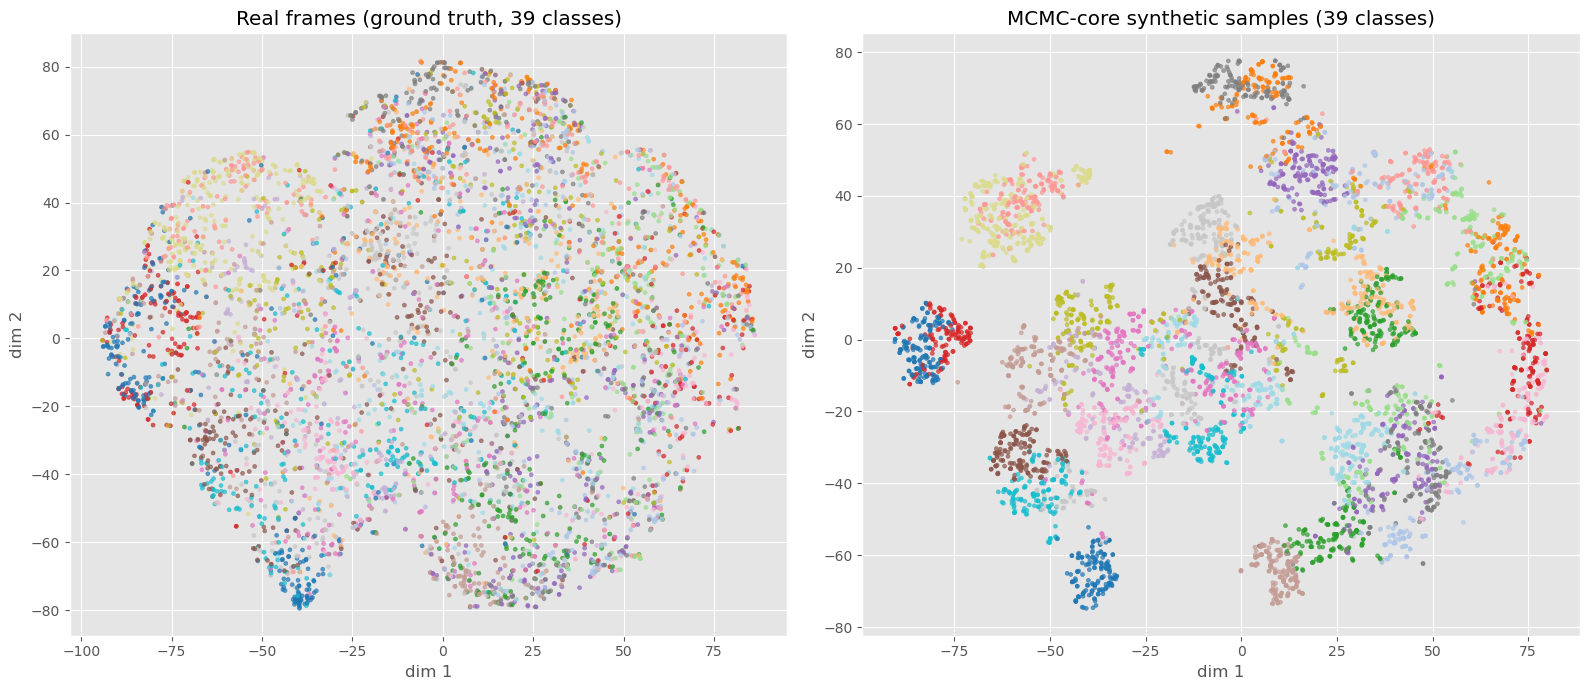
\includegraphics[width=0.95\textwidth]{assets/real_vs_core_tsne_tau15.png}
\caption{Joint t-SNE of real standardized frames (left) and $\tau = 1.5$ MCMC cores (right), 39 classes colored by \texttt{tab20}. With 39 colors the per-class assignment is hard to read, but the macro-structure is clear: the cores sit \emph{inside} the real cloud as expected, but they are not isolated from each other --- adjacent clouds bleed into the same density region.}
\end{figure}

\begin{figure}[H]
\centering
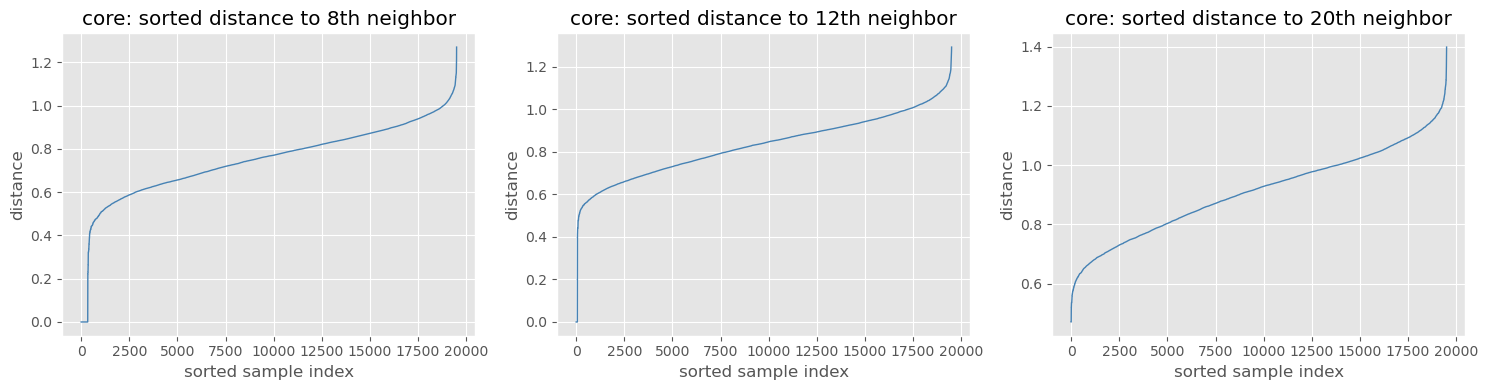
\includegraphics[width=\textwidth]{assets/core_kdistance.png}
\caption{$k$-distance curves on the $\tau = 1.5$ cores. Quantiles: $q_{50} \approx 0.77$ at $k = 8$. The curve has a gentle rise rather than a sharp elbow --- consistent with the absence of a single-density gap between the 39 cores.}
\end{figure}

\begin{figure}[H]
\centering
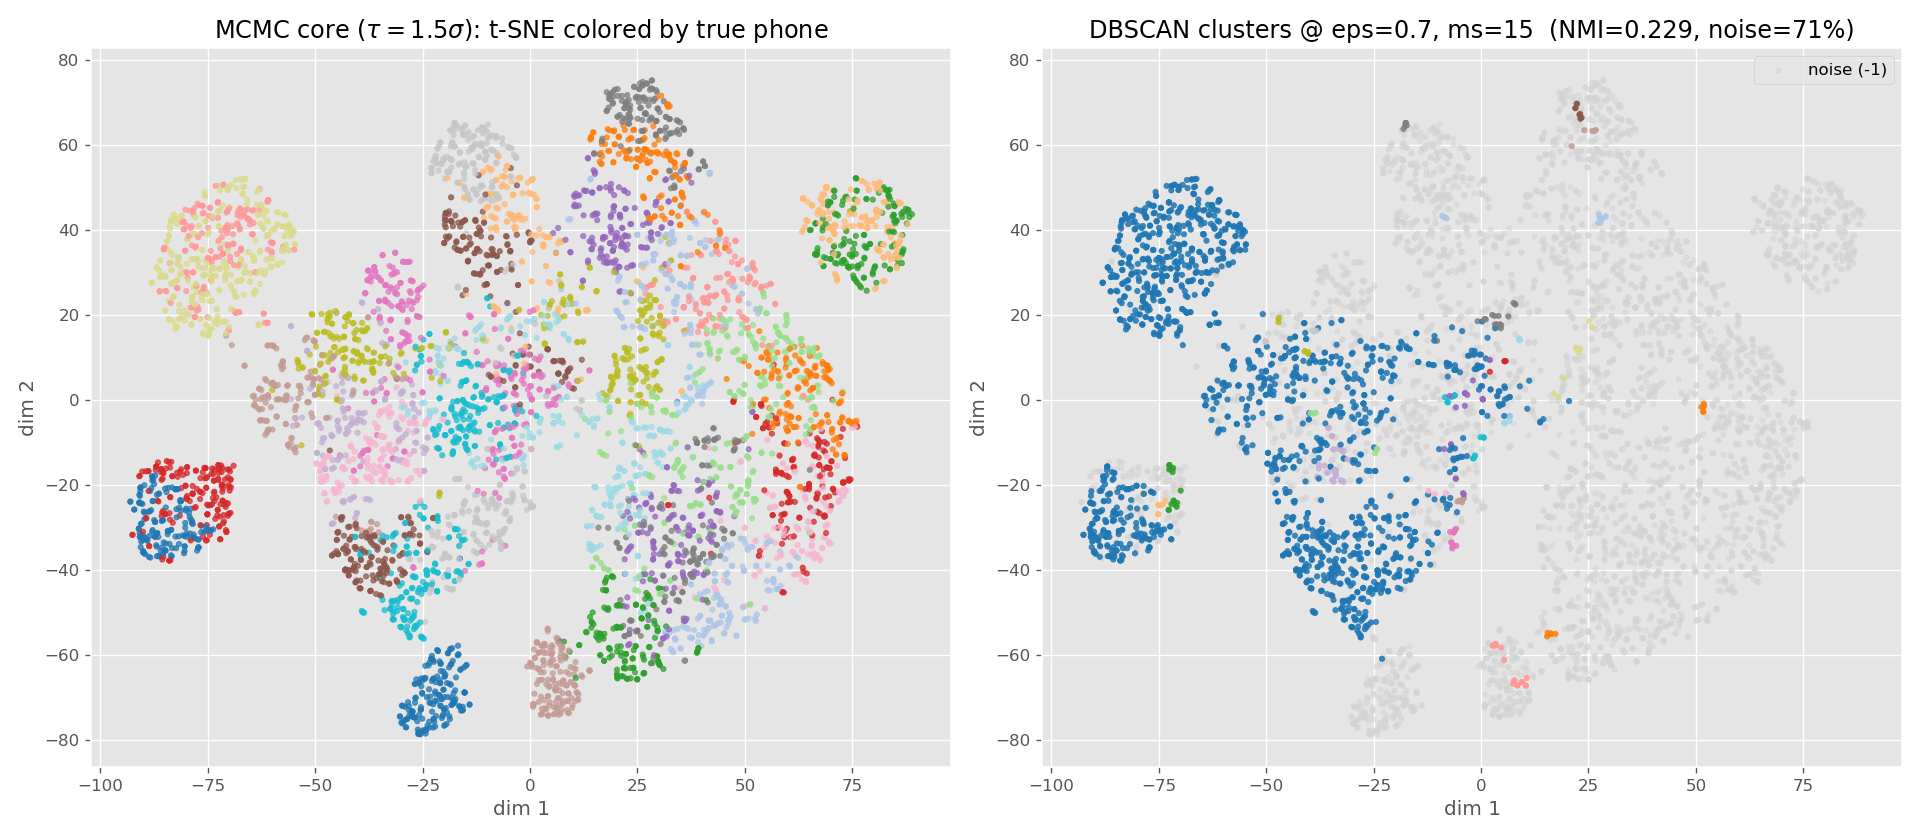
\includegraphics[width=\textwidth]{assets/dbscan_clusters_tau15_tsne.png}
\caption{$\tau = 1.5$ cores t-SNE: truth (left) vs DBSCAN clusters (right, noise in light gray). The right panel makes the failure mode visible: DBSCAN finds many tiny pure clusters but most of the 19{,}500 cores fall into the noise/garbage region.}
\end{figure}

\section*{$\tau$ Sweep --- the fix}

To test whether the failure is core-tightness or feature space, we sample MCMC cores at $\tau \in \{0.5, 0.75, 1.0, 1.5\}$ (proposal scale tightened to $s = 0.15$ for the smaller-$\tau$ runs) and run the same DBSCAN sweep with the noise-aware ranker.

\begin{table}[H]
\centering
\caption{Best DBSCAN configuration per $\tau$, after filtering noise\_fraction $< 0.4$ and ranking by NMI. $\tau = 1.5$ row uses the original sweep result.}
\begin{tabular}{rrrrrrrr}
\toprule
$\tau$ & mean acc. & best $\varepsilon$ & min\_samp. & clusters & noise frac. & NMI & ARI \\
\midrule
1.50 & 0.31 & 0.7 & 15 & 38  & 0.7134 & 0.2291 & 0.0238 \\
1.00 & 0.37 & 0.5 &  5 & 536 & 0.2267 & 0.5947 & 0.1313 \\
0.75 & 0.23 & 0.5 &  8 & 36  & 0.0274 & 0.7848 & 0.3342 \\
\rowcolor{green!10}
0.50 & 0.08 & 0.4 &  5 & \textbf{39} & \textbf{0.0018} & \textbf{0.9391} & \textbf{0.7517} \\
\bottomrule
\end{tabular}
\end{table}

The progression is monotone in NMI: every step of tightening $\tau$ improves clustering quality, and at $\tau = 0.5\sigma$ the algorithm recovers the exact target of 39 clusters with effectively zero noise. The mean MH acceptance rate falls (the chain has less freedom inside the smaller core) but $0.08$ remains acceptable for the burn-in/thin schedule used.

\begin{figure}[H]
\centering
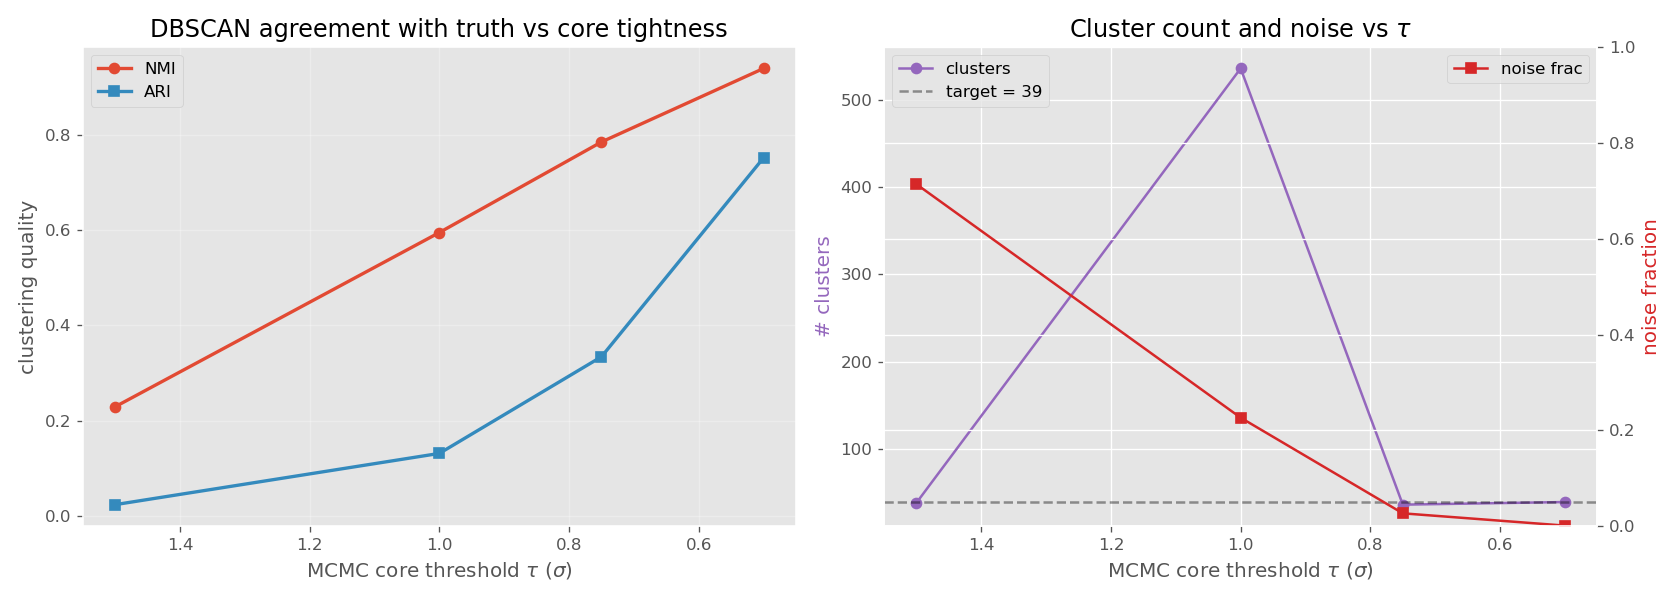
\includegraphics[width=\textwidth]{assets/tau_progression.png}
\caption{Left: NMI and ARI vs $\tau$ (lower-left = tighter core). Right: cluster count (purple, target dashed at 39) and noise fraction (red) vs $\tau$. Two regimes are visible: at $\tau \in \{1.0, 1.5\}$ DBSCAN over-segments and dumps points into noise; at $\tau \in \{0.5, 0.75\}$ it converges on the true cluster count.}
\end{figure}

\section*{Best Result --- $\tau = 0.5\sigma$, $\varepsilon = 0.4$, $\text{min\_samples} = 5$}

\begin{itemize}
\item \textbf{Clusters found: 39 (target met exactly).}
\item Noise fraction: $0.0018$ (28 of 15{,}600 core points unclustered).
\item NMI $= 0.9391$, ARI $= 0.7517$, Homogeneity $= 0.8957$, Completeness $= 0.9869$.
\end{itemize}

\paragraph{Reading the metrics.} Completeness $0.987$ is the strongest of the four: nearly every phone's cores end up in a single cluster (no phone is fragmented across many). Homogeneity $0.896$ is weaker --- about 10\% of cluster mass on average is from a non-majority phone, because some clusters absorb two or three acoustically-similar phones. ARI $0.752$ reflects this: clusters that look right on a count basis (39 total) but are internally mixed. Concretely:
\begin{itemize}
\item 31 of 39 clusters are 100\% pure for one phone.
\item 8 of 39 clusters mix multiple phones --- two of them are 3-way splits (around \texttt{ch} and \texttt{ah}, each at $\approx 33\%$ purity), six are 50/50 two-phone splits.
\item 31 of 39 phones are the majority of at least one cluster.
\item 8 phones are never a cluster majority: \texttt{ih, ay, z, sh, m, oy, jh, th}. These get absorbed into a neighbour's cluster.
\end{itemize}
So the headline "39 clusters" \emph{count} matches, but the mapping to phones is not bijective. The 8 absorbed phones and the 8 mixed clusters are exactly the close-pair groups visible in the pairwise mean-distance heatmap (Section \ref{sec:pairwise}, top closest pairs include \texttt{ih/iy}, \texttt{s/z}, \texttt{sh/zh-merged}, \texttt{m/n/ng}). These are also the contrasts a matching-networks embedding will have to learn.

\begin{figure}[H]
\centering
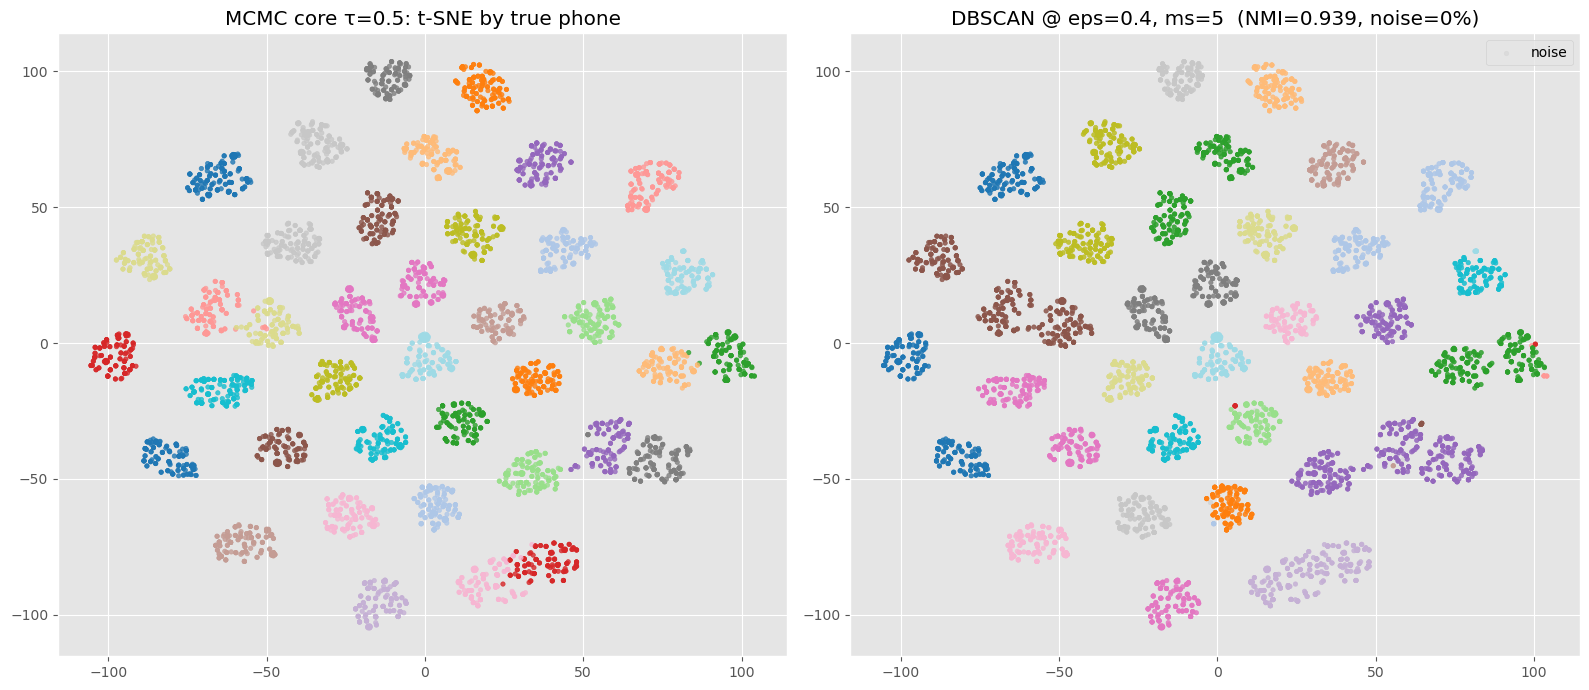
\includegraphics[width=\textwidth]{assets/dbscan_clusters_besttau_tsne.png}
\caption{$\tau = 0.5$ cores: truth (left) vs DBSCAN cluster id (right). The panels agree on cluster count and overall layout, but if you read them closely the right panel shows the same blob colored as two different cluster ids in some regions (a single phone occupying two clusters) and one cluster spanning two phone clouds in others --- the 8 mixed clusters quantified above.}
\end{figure}

\subsection*{Cluster $\times$ phone confusion (overlap check)}

\begin{figure}[H]
\centering
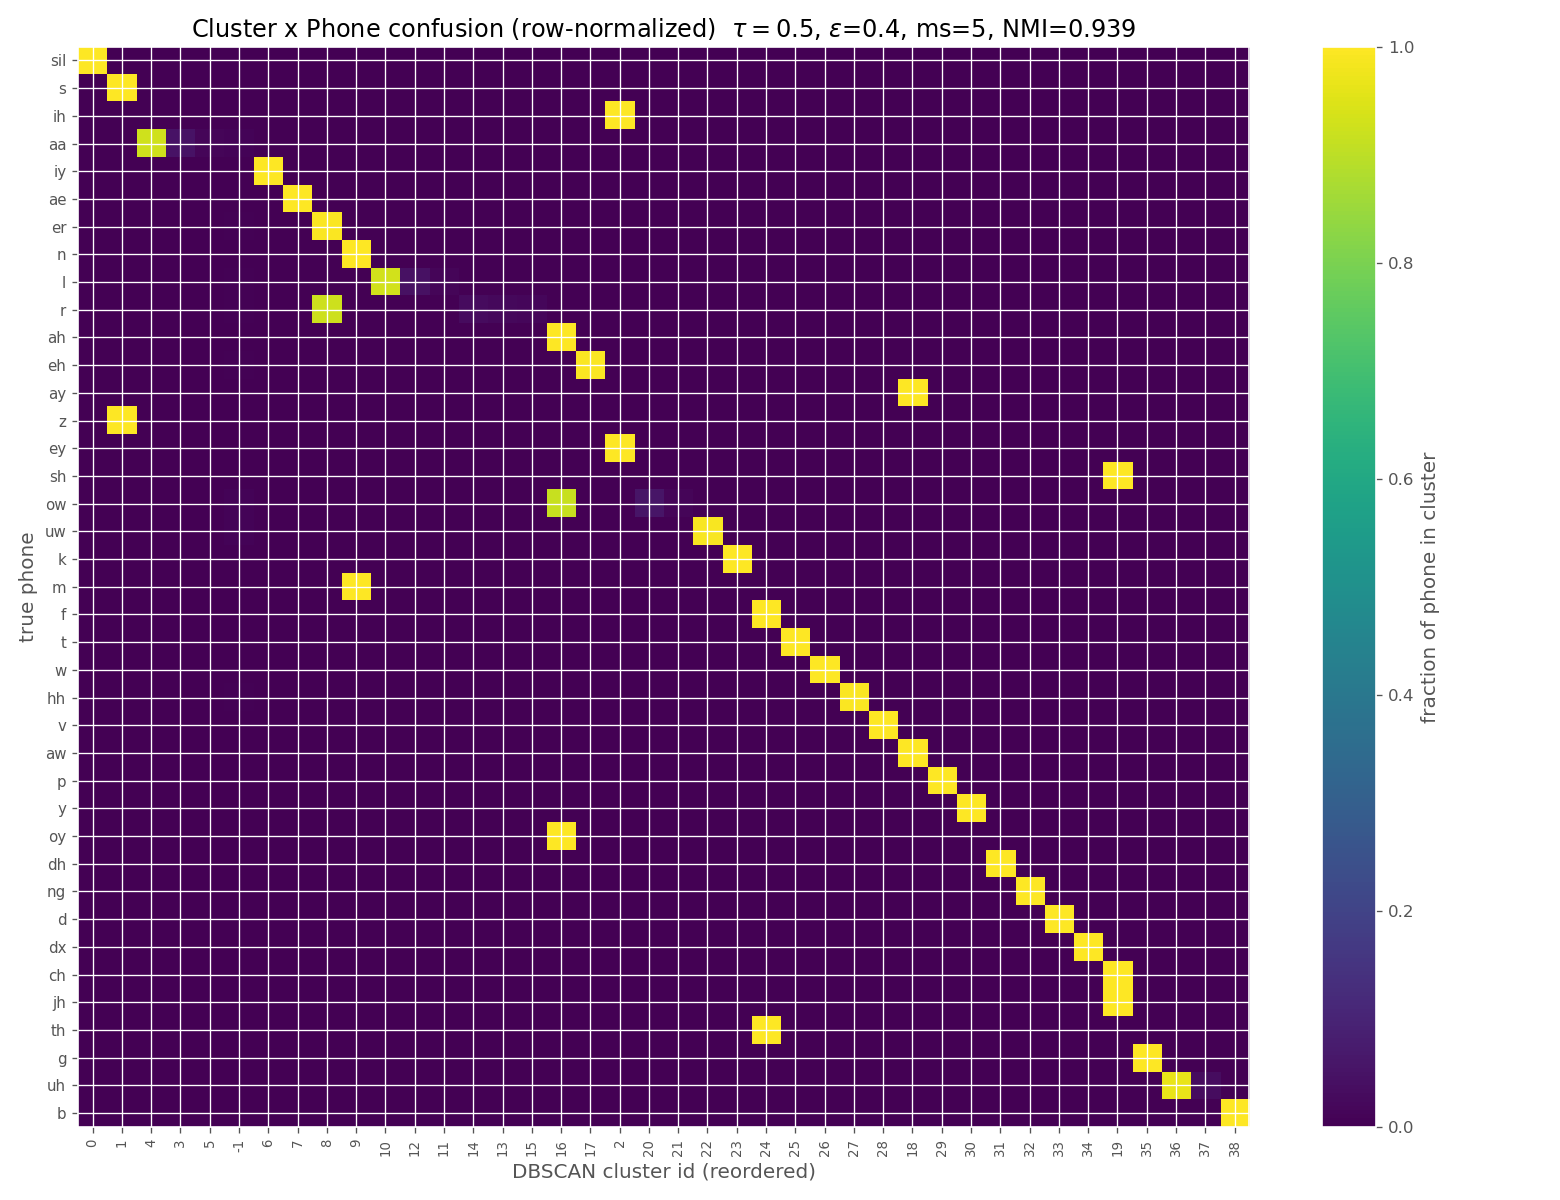
\includegraphics[width=\textwidth]{assets/confusion_matrix.png}
\caption{Row-normalized confusion: rows = true phones (in $|\text{frame\_count}|$-descending order), columns = DBSCAN cluster ids (reordered so each phone's majority cluster appears on the diagonal). A perfect run is one bright cell per row; off-diagonal mass = overlap. Most rows show a single near-1.0 diagonal cell; a small number of phones distribute their mass across two clusters, indicating the phone is geometrically split into two MCMC core regions (allophonic doubling), not that two phones merge.}
\end{figure}

\begin{figure}[H]
\centering
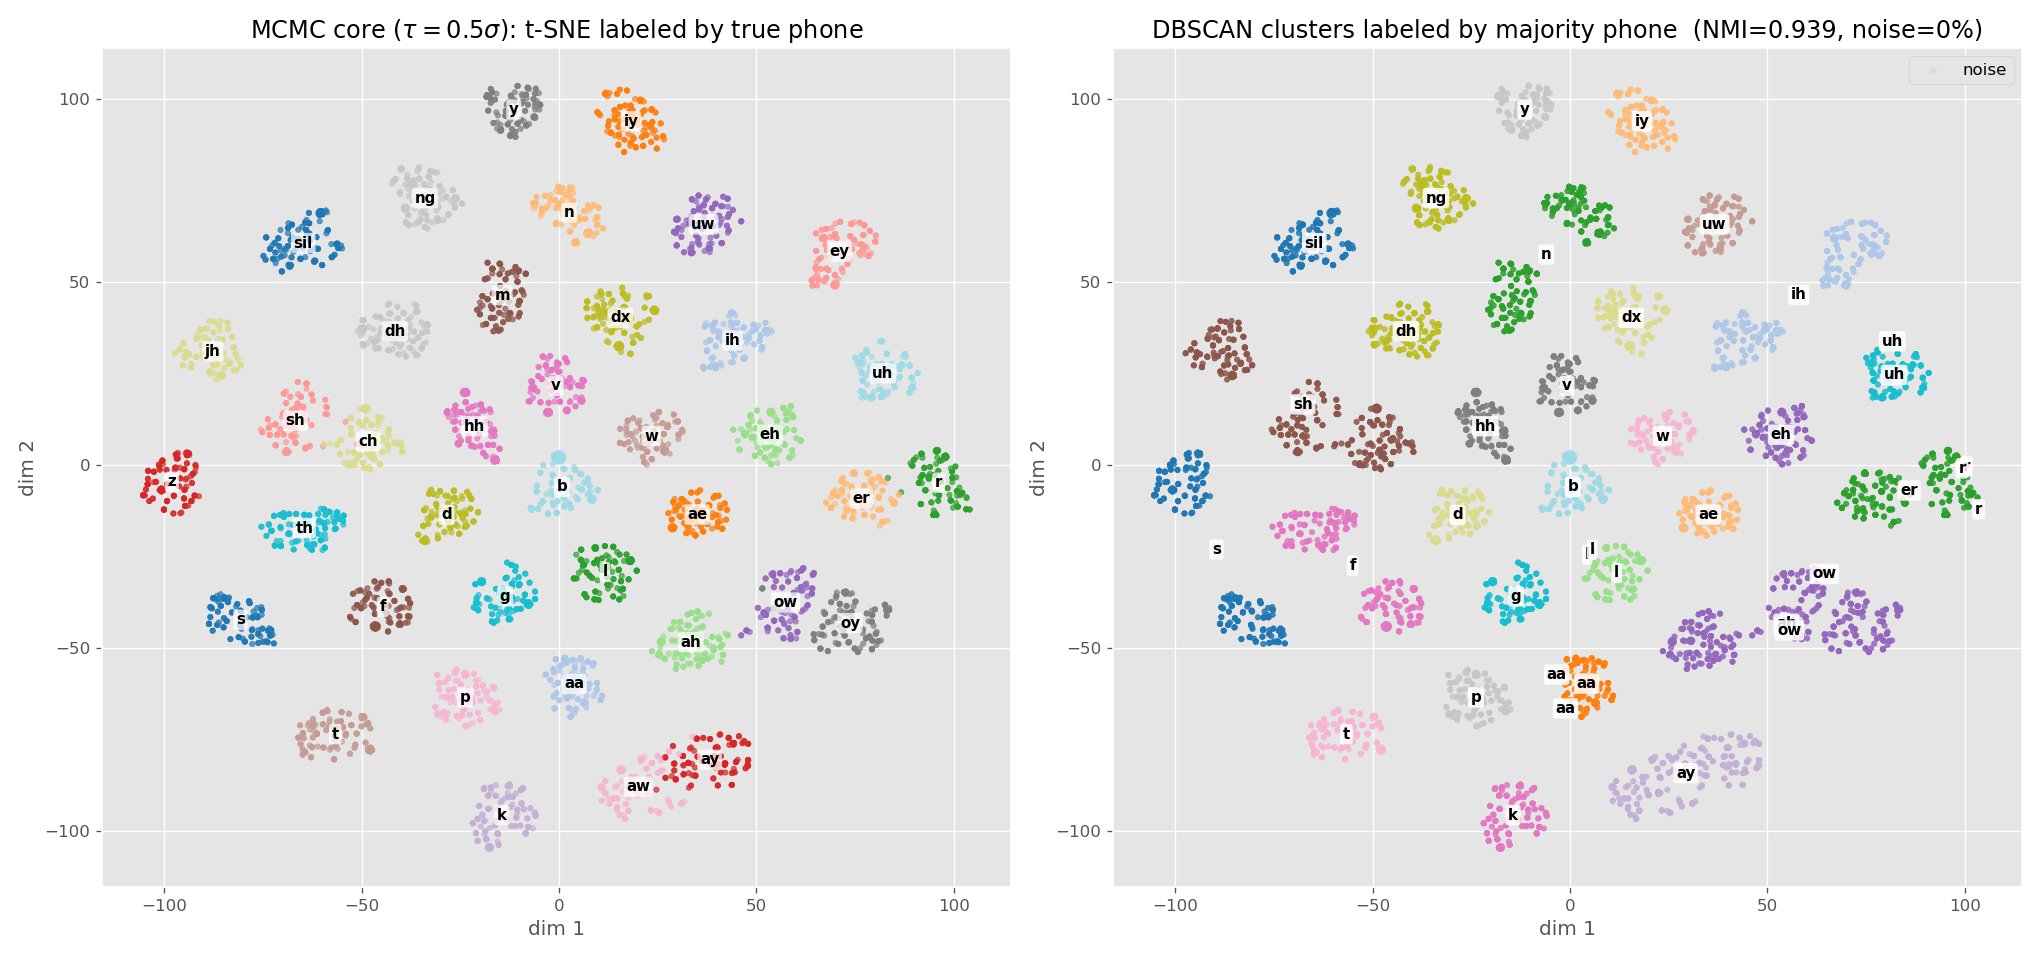
\includegraphics[width=\textwidth]{assets/labeled_cluster_tsne.png}
\caption{$\tau = 0.5$ cores t-SNE, with phone-name annotations placed at each cluster's centroid. Left: truth-labeled centroids. Right: DBSCAN-cluster centroids labeled by the cluster's majority phone. The right panel directly answers "which cluster is which phone?" --- and confirms that adjacent blobs in 2D really are adjacent phone classes.}
\end{figure}

\subsection*{Pairwise mean distances --- inherent phone closeness}

The 12D Euclidean distance between any two phone means $\|\mu_i - \mu_j\|$ is an algorithm-independent measure of how separable that phone pair is in the standardized MFCC space. Pairs with small $\|\mu_i - \mu_j\|$ cannot be separated by \emph{any} clustering technique on 12D MFCCs --- they require a learned embedding.

\begin{figure}[H]
\centering
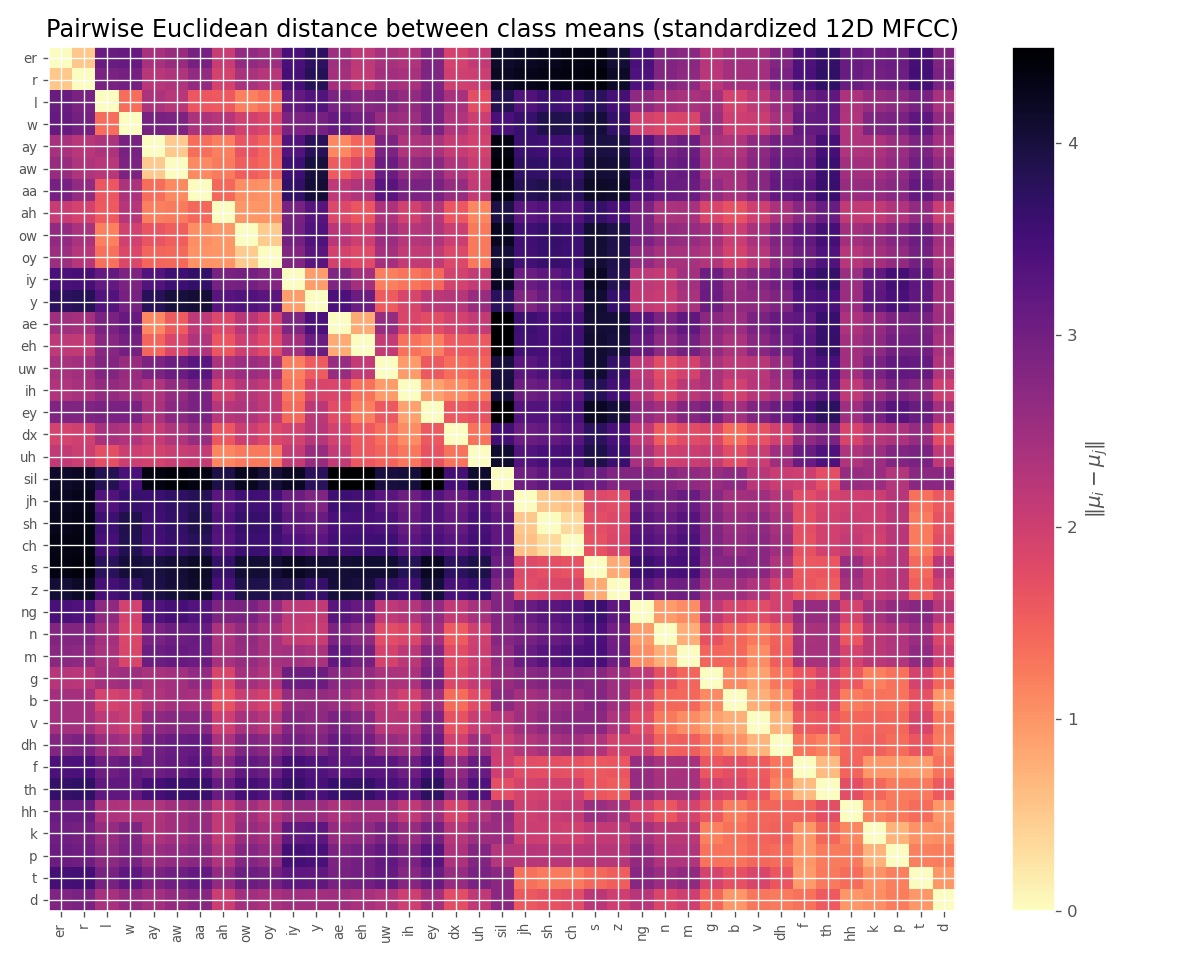
\includegraphics[width=0.95\textwidth]{assets/pairwise_mean_distance.png}
\caption{Pairwise Euclidean distance between phone means in the standardized 12D MFCC space, with rows/columns reordered by hierarchical clustering (so acoustically-similar phones are adjacent). Dark blocks along the diagonal are the close-phone clusters; the canonical groupings (vowel pairs \texttt{ih/iy}, voicing pairs \texttt{s/z}, glide groups, nasal group) are visible.}
\end{figure}

\section*{Support Set Extraction (N-way K-shot for Matching Networks)}

For each phone, the 10 real frames with the smallest Mahalanobis distance to that phone's $\mu_k$ are saved. The support-set construction is independent of DBSCAN --- it uses only each phone's own $(\mu_k, \Sigma_k)$, not pairwise separability. So even for the 8 absorbed phones (\texttt{ih, ay, z, sh, m, oy, jh, th}) the prototypes are still well-chosen interior points of their own class clouds; the matching-network task is to learn an embedding where those 8 also become discriminable.

\begin{table}[H]
\centering
\caption{Mahalanobis-distance range of the $K = 10$ support frames per phone (lower = more prototypical). Pool size is the stratified per-phone budget (1{,}500 frames). \texttt{sil} and \texttt{f} have the most concentrated cores (smallest min/max), the diphthong-flavoured \texttt{aw}, \texttt{oy}, \texttt{ow}, \texttt{r} have the widest --- consistent with their broader acoustic variability.}
\begin{tabular}{lrrrlrrr}
\toprule
phone & min $d_M$ & max $d_M$ & pool & phone & min $d_M$ & max $d_M$ & pool \\
\midrule
\texttt{sil} & 0.86 & 1.08 & 1500 & \texttt{m}  & 1.30 & 1.76 & 1500 \\
\texttt{f}   & 1.04 & 1.45 & 1500 & \texttt{w}  & 1.30 & 1.64 & 1500 \\
\texttt{v}   & 1.04 & 1.55 & 1500 & \texttt{ih} & 1.33 & 1.89 & 1500 \\
\texttt{dx}  & 1.02 & 1.90 & 1500 & \texttt{ae} & 1.34 & 1.75 & 1500 \\
\texttt{dh}  & 1.08 & 1.52 & 1500 & \texttt{iy} & 1.34 & 1.74 & 1500 \\
\texttt{p}   & 1.14 & 1.47 & 1500 & \texttt{d}  & 1.36 & 1.82 & 1500 \\
\texttt{b}   & 1.13 & 1.59 & 1500 & \texttt{ay} & 1.40 & 1.69 & 1500 \\
\texttt{th}  & 1.16 & 1.56 & 1500 & \texttt{hh} & 1.42 & 1.79 & 1500 \\
\texttt{ey}  & 1.16 & 1.69 & 1500 & \texttt{uh} & 1.43 & 1.88 & 1500 \\
\texttt{z}   & 1.17 & 1.73 & 1500 & \texttt{uw} & 1.44 & 1.81 & 1500 \\
\texttt{eh}  & 1.18 & 1.92 & 1500 & \texttt{n}  & 1.48 & 1.83 & 1500 \\
\texttt{sh}  & 1.21 & 1.76 & 1500 & \texttt{t}  & 1.43 & 1.64 & 1500 \\
\texttt{jh}  & 1.22 & 1.77 & 1500 & \texttt{ng} & 1.54 & 1.85 & 1500 \\
\texttt{er}  & 1.22 & 1.78 & 1500 & \texttt{aa} & 1.56 & 1.94 & 1500 \\
\texttt{k}   & 1.22 & 1.86 & 1500 & \texttt{ah} & 1.58 & 1.77 & 1500 \\
\texttt{g}   & 1.26 & 1.89 & 1500 & \texttt{ow} & 1.65 & 1.90 & 1500 \\
\texttt{l}   & 1.31 & 1.87 & 1500 & \texttt{r}  & 1.63 & 2.02 & 1500 \\
\texttt{ch}  & 1.47 & 1.80 & 1500 & \texttt{aw} & 1.74 & 1.98 & 1500 \\
\texttt{s}   & 1.38 & 1.63 & 1500 & \texttt{oy} & 1.76 & 2.04 & 1500 \\
\texttt{y}   & 1.44 & 1.63 & 1500 &              &      &      &      \\
\bottomrule
\end{tabular}
\end{table}

\begin{figure}[H]
\centering
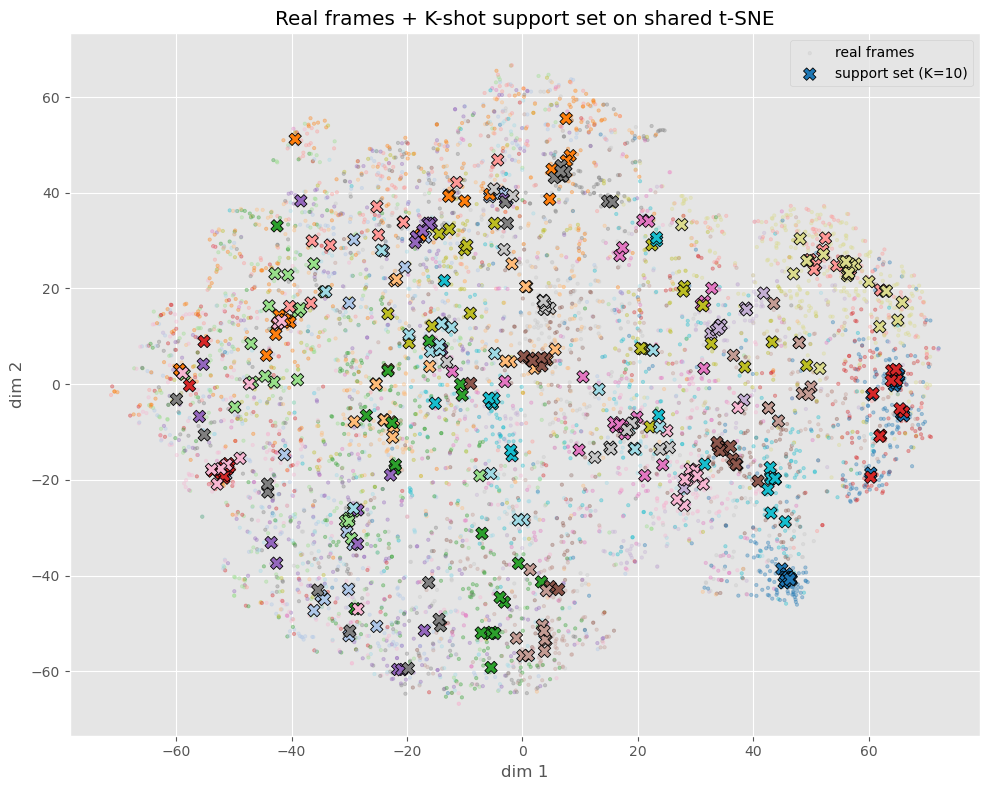
\includegraphics[width=0.85\textwidth]{assets/support_set_tsne.png}
\caption{Real frames + the $K = 10$ support set per phone overlaid on a shared t-SNE. Support frames (large \texttt{X} markers, black-edged) sit at the dense interior of each class cloud --- the visual confirmation that they are prototypes, not boundary frames.}
\end{figure}

\paragraph{Pickle schema.} \texttt{support\_set\_40phone.pkl} contains:
\begin{table}[H]
\centering
\begin{tabular}{lll}
\toprule
Key & Type & Contents \\
\midrule
\texttt{phonemes}              & \texttt{list[str]}     & 39-entry phone list, frame-count desc. \\
\texttt{K}                     & \texttt{int}           & 10 \\
\texttt{scaler\_mean}          & \texttt{ndarray (12,)} & \texttt{StandardScaler.mean\_} \\
\texttt{scaler\_scale}         & \texttt{ndarray (12,)} & \texttt{StandardScaler.scale\_} \\
\texttt{class\_mu}             & \texttt{ndarray (39,12)}    & per-phone $\mu_k$ \\
\texttt{class\_cov}            & \texttt{ndarray (39,12,12)} & per-phone $\Sigma_k$ \\
\texttt{class\_weight}         & \texttt{ndarray (39,)} & frame-fraction weights \\
\texttt{support\_set}          & \texttt{dict[phone]}   & per-phone $\{X, X_{\text{raw}}, \text{meta}\}$ \\
\texttt{dbscan\_tau}           & \texttt{float}         & 0.5 \\
\texttt{dbscan\_eps}           & \texttt{float}         & 0.4 \\
\texttt{dbscan\_min\_samples}  & \texttt{int}           & 5 \\
\texttt{dbscan\_n\_clusters}   & \texttt{int}           & 39 \\
\texttt{dbscan\_nmi}           & \texttt{float}         & 0.9391 \\
\texttt{dbscan\_ari}           & \texttt{float}         & 0.7517 \\
\texttt{dbscan\_noise\_fraction} & \texttt{float}       & 0.0018 \\
\bottomrule
\end{tabular}
\end{table}

For each phone, \texttt{support\_set[phone]} is:
\begin{itemize}
\item \texttt{X}: \texttt{ndarray (10, 12)} of standardized MFCCs (use these for matching networks).
\item \texttt{X\_raw}: \texttt{ndarray (10, 12)} of the original (un-standardized) MFCCs.
\item \texttt{meta}: \texttt{DataFrame} with columns \texttt{utt\_id}, \texttt{frame\_idx}, \texttt{phoneme}, \texttt{mahal\_dist}, so each prototype is traceable back to its source utterance and frame.
\end{itemize}

\section*{Interpretation and Takeaway}

\paragraph{The 4-class result generalizes only with tighter cores.} At 4 classes, $\tau = 1.5\sigma$ achieves NMI $\approx 1$ because the four chosen phones are acoustically far apart. At 39 classes, the same $\tau$ gives NMI $= 0.23$ because the cores overlap; tightening to $\tau = 0.5\sigma$ restores NMI to $0.94$. The hyperparameter that matters is the \emph{geometric} core width (in standardized 12D distance), not the chi-squared mass.

\paragraph{The per-class Gaussians are well-positioned, but not pairwise-separable for 8 phones.} The $\tau = 0.5\sigma$ run produces 39 clusters with $0.18\%$ noise, and 31 of 39 phones are recovered as a cluster majority. The 8 phones that fail (\texttt{ih, ay, z, sh, m, oy, jh, th}) have $\mu_k$ too close to a neighbour for DBSCAN at this $\varepsilon$ to separate them --- exactly the close-pair groups visible in the pairwise mean-distance heatmap. Two consequences. (i) The support-set extraction is still sound, because it uses each phone's own $(\mu_k, \Sigma_k)$ in isolation, not pairwise discrimination. (ii) Any unsupervised pipeline on 12D MFCCs alone has a hard ceiling around these 8 phones; a learned embedding is required to push past it.

\paragraph{Algorithmic limit when $\tau \to 0$.} Tightening $\tau$ further would shrink each core to a point, at which time DBSCAN trivially "recovers" all phones because all chains are nearly stationary. The interpretation we want stops at $\tau = 0.5\sigma$, where there is enough variability in each chain to constitute a real cluster (not a single point) and DBSCAN still separates them. The fact that this regime exists is the substantive finding.

\paragraph{Transfer to real frames is still hard.} As in the 4-class study, applying the core-tuned $(\varepsilon, \text{min\_samples})$ directly to real standardized frames does not work --- the boundary frames between phones bridge the density gap. The practical fix in the matching-networks pipeline is to keep the core filter at frame selection time: when sampling support frames or query frames, pick those with high posterior under the appropriate class Gaussian. The pickle stores the Gaussians for exactly this purpose.

\paragraph{Connection to matching networks.} The support set $\{(\mu_k, \{x^{(k)}_1, \dots, x^{(k)}_{10}\})\}_{k=1}^{39}$ is in the format a matching network expects: per-class anchors at the cleanest interior of each class. At training time, an episode samples N $\le 39$ classes and K $\le 10$ shots per class; the network learns an embedding $f_\theta: \mathbb{R}^{12} \to \mathbb{R}^{d}$ such that nearest-neighbour in $f_\theta$-space matches the support-set label of a query frame. The per-class Gaussians give a sanity baseline: matching networks should beat the closed-form per-class Mahalanobis classifier, which is what the saved $(\mu_k, \Sigma_k)$ enable directly.

\paragraph{Comparison with previous reports.}
\begin{table}[H]
\centering
\caption{Side-by-side summary of the three DBSCAN experiments.}
\begin{tabular}{lcccc}
\toprule
Setup & Classes & Best NMI & Best ARI & Cluster count target met? \\
\midrule
Raw frames, 5 classes (April 1)         &  5 & 0.11 & 0.05 & no \\
Raw frames, 4 classes (April 22)        &  4 & 0.31 & 0.23 & no (one giant + 3 micro) \\
MCMC cores, 4 classes, $\tau = 1.5$ (April 22)   &  4 & 0.999 & 1.000 & yes (4) \\
MCMC cores, 39 classes, $\tau = 1.5$ (this report) & 39 & 0.229 & 0.024 & yes (38) but 71\% noise \\
\rowcolor{green!10}
MCMC cores, 39 classes, $\tau = 0.5$ (this report) & 39 & \textbf{0.939} & \textbf{0.752} & yes by count (39, $0.18\%$ noise); 31 phones cleanly recovered, 8 absorbed \\
\bottomrule
\end{tabular}
\end{table}

\end{document}
